\documentclass[14pt,a4paper]{scrartcl}
\usepackage[utf8]{inputenc}
\usepackage[russian]{babel}
\usepackage[T2]{fontenc}
\usepackage[warn]{mathtext}
\usepackage{graphicx}
\usepackage{amsmath}Ч
\usepackage{floatflt}
\usepackage[left=20mm, top=20mm, right=20mm, bottom=20mm, footskip=10mm]{geometry}


\graphicspath{ {images/} }
\usepackage{multicol}
\setlength{\columnsep}{2cm}


\begin{document}

\begin{titlepage}
	 \begin{center}
    \large
    МИНИСТЕРСТВО ОБРАЗОВАНИЯ И НАУКИ\\ РОССИЙСКОЙ ФЕДЕРАЦИИ
     
    \vspace{0.5cm}
 
    Федеральное государственное автономное образовательное учреждение высшего образования \\ «МОСКОВСКИЙ ФИЗИКО-ТЕХНИЧЕСКИЙ ИНСТИТУТ (научно-исследовательский институт)»
    \vspace{0.25cm}

  Физтех-школа аэрокосмических технологий
     
    Кафедра общей физики
    \vfill
     
     

    
    Плотников Святослав Иванович
    \vfill
 
     
    {\LARGE Моделирование оптических приборов и определение их увеличения\\}
     
   2 курс, группа Б03-901
\end{center}
\vfill

\vfill
 
\begin{center}
  Долгопрудный, 2021 г.
\end{center}
\end{titlepage}


\tableofcontents
\addcontentsline{exp}{section}{Заголовок добавить в содержание}
\newpage


\section{Цель работы:}
Изучить модели зрительных труб (астрономической трубы Кеплера и земной трубы Галилея) и микроскопа, определить их увеличения

\section{В работе используются:}
\begin{itemize}
    \item оптическая скамья
    \item набор линз
    \item экран
    \item осветитель со шкалой
    \item зрительная труба
    \item диафрагма
    \item линейка.
\end{itemize}

\newpage
\section{Теоретические сведения:}
\subsection{Телескоп Кеплера}

В телескопе Кеплера используются две тонкие собирающие линзы с фокусными расстояниями $f_1, f_2$, , расположенные на расстоянии $l_{12}=f_{1}+f_{2}$ друг от друга. Он предназначен для наблюдения удаленных предметов. Угловое увеличение телескопа Кеплера равно $$N_{T}=-\frac{f_{1}}{f_{2}}$$
\begin{center}
  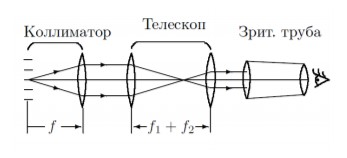
\includegraphics[width = 7cm]{труба кеплера.jpg}\\
  Рис. 1 Схема установки для определения увеличения телескопа Кеплера
 
\end{center}

\begin{center}
  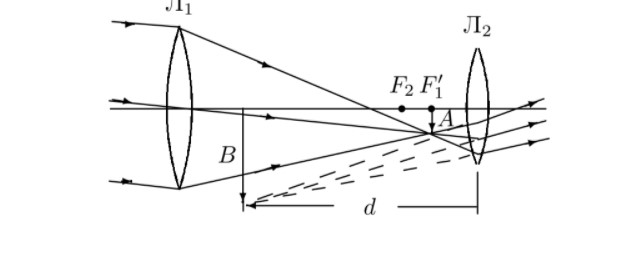
\includegraphics[width = 9cm]{ход лучей в кеплере.jpg}\\
  Рис. 2 Ход лучей в трубе Кеплера,
Л1 - объектив, Л2 - окуляр
\end{center}




\subsection{Телескоп Галлилея}

В зрительной трубе Галлилея в качестве окуляра вместо собирающей линзы используется
рассеивающая. Угловое увеличение тоже самое:
$$N_{T}=-\frac{f_{1}}{f_{2}}$$

\begin{center}
  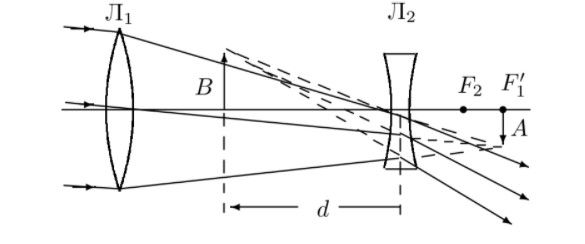
\includegraphics[width = 8cm]{ход лучей в гал.jpg}\\
  Рис. 3 Ход лучей в зрительной трубе Галилея
 
\end{center}


\subsection{Микроскоп}
Микроскоп состоит из двух собирающих линз - объектива и окуляра, расположенных на
расстоянии $l_{12}$ друг от друга. Наблюдаемый предмет помещается на малом расстоянии
перед передним фокусом объектива. Обозначим $\Delta=l_{12}-f_{1}-f_{2}$ оптический интервал, $L$ - расстояние наилучшего зрения. Увеличение микроскопа равно
$$
N_{M}=-\frac{\Delta L}{f_{1} f_{2}}
$$


\begin{center}
  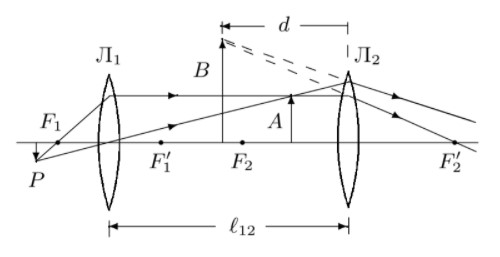
\includegraphics[width = 8cm]{ход лучей в микроскопе.jpg}\\
  Рис. 4 Ход лучей в зрительной трубе Галилея
 
\end{center}


\begin{center}
  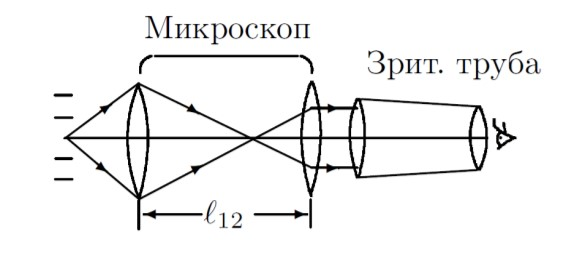
\includegraphics[width = 8cm]{Схема установки для определения увеличения микроскопа.jpg}\\
  Рис. 5 Схема установки для определения увеличения микроскопа
 
\end{center}





\section{Определение фокусных расстояний линз с помощью зрительной трубы}
Настроим зрительную трубу на бесконечность. Найдем фокусные расстояния собирающих
линз, расположив их на расстоянии, приблизительно равном фокусному, от предмета и
глядя на них через зрительную трубу. Мы увидим четкое изображение, когда расстояние
от линза до предмета равно фокусному. Фокусное расстояние рассеивающей линзы можно
найти, расположив ее за собирающей линзой с известным фокусным расстоянием. Фокусное расстояние находится по формуле $F=l-a_{0}$







    
































\begin{center}
\begin{tabular}{|l|l|l|l|}
\hline
n & $F_{1}$, см & $F_{2}$, см & $F_{3}$,см \\ \hline
1 & 7.6    & 7.8    & 7.7  \\ \hline
2 & 10.2   & 10.4   & 10.3 \\ \hline
3 & 19.4   & 19.6   & 19.5 \\ \hline
4 & 28.2   & 27.8   & 28.0 \\ \hline
5 & -9.2   & -9.0   & -9.1 \\ \hline
\end{tabular}

\end{center}
\begin{center}
Таблица 1: Фокусные расстояния линз
\end{center}

\section{Моделирование трубы Кеплера}
\begin{enumerate}
    \item Рассмотрим ход лучей в трубе Кеплера и найдём увеличение данной оптической системы. Соберем установку, изображенную на рисунке 1.
    \item Для коллиматора будем использовать
линзу с фокусным расстоянием $f_{k}=19.5 \pm 0.4$см. для объектива $f_{1}=28.0 \pm 0.4$см.
для окуляра $f_{2}=10.3 \pm 0.4$см. пределим размер одного деления шкалы осветителя в
единицах шкалы зрительной трубы. Результат равен $h_{1}=0.72  \pm  0.02$см.

Рассчитаем увеличение телескопа через фокусные расстояния линз.

$$
N_{T, 1}=-\frac{f_{1}}{f_{2}}=2.71 \pm 0.14
$$
С помощью зрительной трубы измерим угловой размер $h_{2}$ деления изображения источника. Результат равен
$$
h_{2}=2.10 \pm 0.05
$$

Увеличение телескопа, измеренное этим методом, равно

$$
N_{T, 2}=-\frac{h_{2}}{h_{1}}=2.86 \pm 0.15
$$

Другой способ определения увеличения - по отношению диаметра оправы объектива и
диаметра изображения этой оправы в окуляре. Диаметр оправы равен $D_{1}=3.8 \pm 0.1$ см, диаметр ее изображения - $D_{2}=1.4 \pm 0.1$
Тогда увеличение микроскопа равно $N_{T, 3}=-\frac{D_{1}}{D_{2}}=-2.76 \pm 0.3$
\end{enumerate}


\section{Моделирование трубы Галилея}
    \begin{enumerate}
    \item Ход лучей в микроскопе показан на рис. 6. Увеличение микроскопа вычисляется по формуле
 Заменим телескоп Кеплера на трубу Галилея. Для этого вместо собирающей линзы окуляра поставим рассеивающую линзу на расстоянии от объектива, равном сумме фокусных расстояний. Фокусное расстояние объектива равно 
 $f_{1}=28.0 \pm 0.4$см, окуляра $f_{2}=-9.1 \pm 0.6$см
 
 Увеличение трубы Галилея, найденное из фокусных расстояний линз, равно
 $$
N_{\Gamma, 1}=-\frac{f_{1}}{f_{2}}=3.1 \pm 0.3
$$
Измерим видимый угловой размер h2 деления осветителя.

$$
h_{2}=2.25 \pm 0.05
$$

Увеличение равно
$$
N_{\Gamma, 2}=\frac{h_{2}}{h_{1}}=3.04 \pm 0.15
$$
 \end{enumerate}
\begin{enumerate}

\end{enumerate}

\section{Моделирование микроскопа}
Соберем модель микроскопа, изображенную на рисунке 5. Параметры установки: 
$f_{1}=7.7 \pm 0.4$см, $f_{2}=10.3 \pm 0.4$см, $l_{12}=33.3 \pm 0.2$см
\begin{enumerate}
Увеличение равно: 
$$
N_{M, 1}=-\frac{\left(l_{12}-f_{1}-f_{2}\right) L}{f_{1} f_{2}}=-4.9 \pm 0.7
$$
   
   
   Измерим видимый угловой размер h2 деления осветителя.
   $$
h_{2}=2.50 \pm 0.05
$$

Увеличение микроскопа
$$
N_{M, 2}=-\frac{h_{2} L}{h_{1} f}=-4.4 \pm 0.3
$$
Различие между увеличениями, найденными двумя способами, остаются в пределах
погрешностей.
\end{enumerate}

\section{Вывод}
В работе были собраны модели телескопа Кеплера, трубы Галилея и микроскопа. Были
найдены их увеличения из параметров установки, а также из отношения угловых размеров
источника и его изображения. Все различия между результатами оказались в пределах
погрешностей.

    
\end{document}